
\chapter{ANALYSIS}
\label{Chapter:Analysis}

\emph{This section is under development and it will expand as I continue my experiments and implementation.}

\section{Security}

Now we examine and compare OnioNS's central protocols against our security assumptions and expected threat model.

\subsection{Hidden Service Protocols}

\subsubsection{Record Generation}

The Record Generation protocol can safely take place within an offline machine under the operator's control. We designed the protocol to require resigning the Record fields after every round of scrypt so as to require the owner of the private key to also perform the scrypt proof-of-work. Scrypt introduces a cost and its memory demands increases the difficulty of custom hardware and massively-parallel attacks, effectively limiting adversaries to the same hardware as legitimate users. 

However, our protocol does not entirely prevent a hidden service operator from outsourcing the computation to secondary resource. Let Bob be the hidden service and Craig the owner of the computational resource. We assume that Craig does not have Bob's private key. Then,

\begin{enumerate}
	\item Bob creates an initial Record $ R $ and completes the \emph{type}, \emph{nameList}, \emph{contact}, \emph{timestamp}, and \emph{consensusHash} fields.
	\item Bob sends $ R $ to Craig.
	\item Let $ \mathit{central} $ be $\mathit{type} \concat \mathit{nameList} \concat \mathit{contact} \concat \mathit{timestamp} \concat \mathit{consensusHash} \concat \mathit{nonce} $.
	\item Craig generates a random integer $ K $ and then for each iteration $ j $ from 0 to $ K $,
		\begin{enumerate}
			\item Craig increments \emph{nonce}.
			\item Craig sets \emph{PoW} as $ \mathrm{PoW}(\mathit{central}) $.
			\item Craig saves the new $ R $ as $ C_{j} $.
		\end{enumerate}
	\item Craig sends all $ C_{0 \le j \le K} $ to Bob.
	\item For each Record $ C_{0 \le j \le K} $ Bob computes
		\begin{enumerate}
			\item Bob sets \emph{pubHSKey} to his public RSA key.
			\item Bob sets \emph{recordSig} to $ S_{d}(m, r) $ where $ m = \mathit{central} \concat \mathit{pow} $ and $ r $ is Bob's private RSA key.
			\item Bob has found a valid record if $ H(\mathit{central} \concat \mathit{pow} \concat \mathit{recordSig}) \leq 2^{\mathit{difficulty} * \mathit{count}} $
		\end{enumerate}
\end{enumerate}

% todo: calculate chances of Craig computing a correct record

Our protocol ensures that Craig must always compute more scrypt iterations than necessary; Craig cannot generate \emph{recordSig} and thus cannot compute if the hash is below the threshold. Moreover, the scrypt work incurs a cost onto Craig that must be compensated financially by Bob. Thus the Record Generation protocol places a lower bound on the cost paid by Bob.

\subsubsection{Record Broadcast}

\emph{Todo: what are the implications of Bob sending his Record to a malicious Quorum node?}

A Tor circuit is used to protect Bob's privacy during Record Broadcast.

\subsection{OnioNS Server Protocols}

\subsubsection{Page Selection}

\emph{What are the implications of the whole Quorum being malicious? Can the network be misled? What are the chances of that occurring? Page Selection seems dependent on the Quorum's last flood.}

\subsubsection{Synchronization}

\emph{What could a Mirror lie about, and what are the implications? I'm really not sure what could happen here because of the Page signatures.}

\subsubsection{Quorum Qualification}

\emph{I am still analysing the statistics of an attacker gaining control of the Quorum, assuming all of their machines collude. We explore the optimal Quorum rotation rate, given the balance between high overhead and high security risk if the Quorum is rotated quickly, and long-term implications and possible stability issues associated with very slow rotation.}

The Quorum holds the greatest amount of responsibility over OnioNS and they likewise have greater attack capabilities than any other class of participants in OnioNS. In a Tor network of $ N = 5400 $ routers, we assume that Eve controls some fixed fraction $ x $ of them. The chance of Eve controlling more than half of the Quorum and the Pagechain assuming all of her machines collude is given by the summation of the hypergeometric distribution, $ \displaystyle\sum_{x=\ceil{\frac{n}{2}}}^{n} \frac{\binom{n}{k}\binom{N-k}{n-x}}{\binom{N}{n}} $. We graph this distribution for $ N $ routers in Figure \ref{chart:quorumMajority}.

\begin{figure}[htbp]
	\centering
	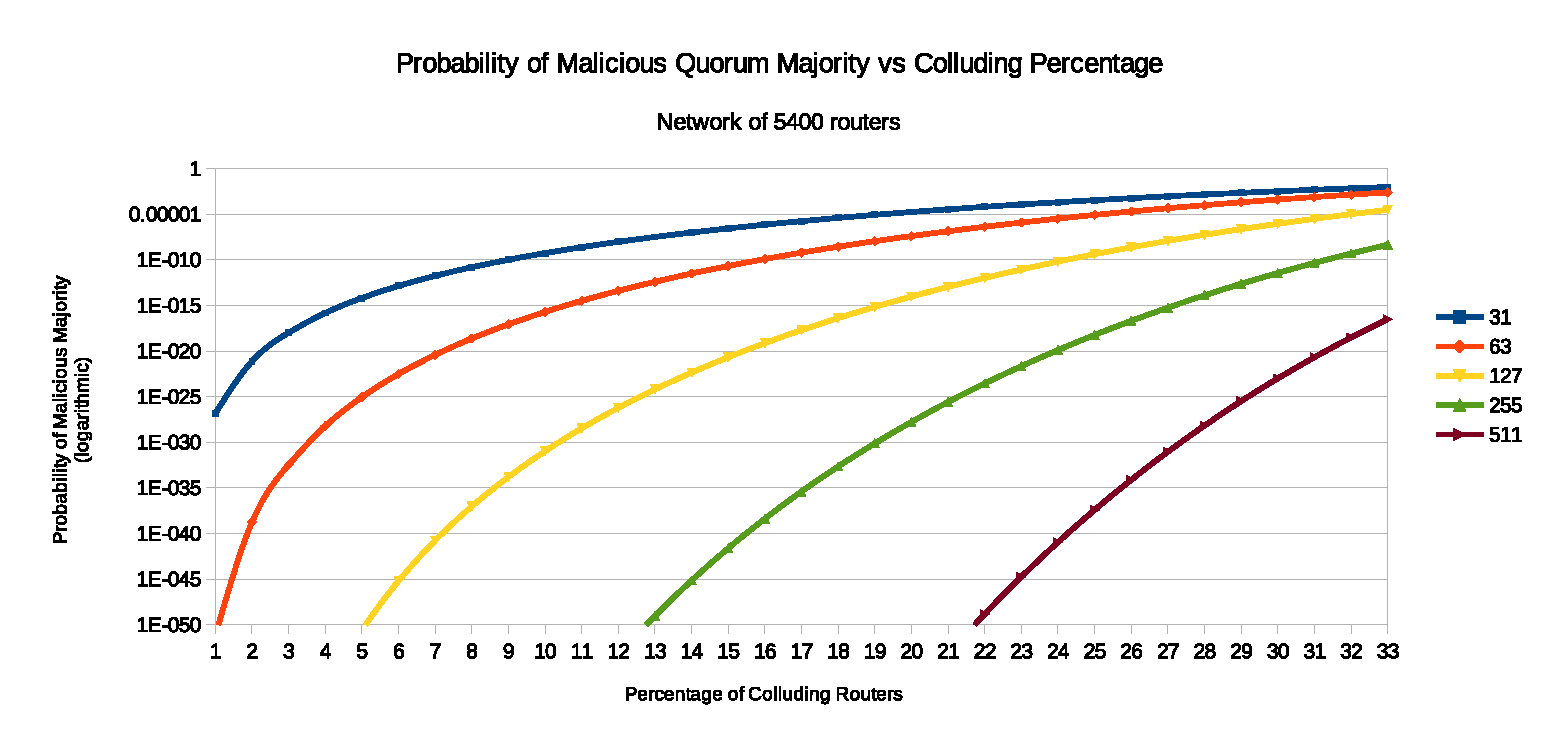
\includegraphics[width=0.95\textwidth]{images/QuorumMajorityProbability.eps}
	\caption{We assume that Eve controls some percentage of potentially-colluding nodes on the Tor network. This chart represents the probability (given by the summation of hypergeometric distribution) that half or more of the Quorum is Eve's control, on a network of 5,400 nodes and Quorum sizes of 31, 63, 127, and 511. If the majority of the Quorum is controlled in this way, it represents a complete compromise of the Quorum's integrity as Eve's Pages will always be selected regardless of the behavior of the rest of the Quorum.}
	\label{chart:quorumMajority}
\end{figure}

1/256 = 10^-77.064

1/192 = 10^-57.798

1/128 = 10^-38.532

If Eve controls some Tor nodes (who may be assumed to be colluding with one another), the attacker may desire to include their nodes in the Quorum for malicious manipulation, passive observation, or for other purposes. Alternatively, Eve may wish to exclude certain legitimate nodes from inclusion in the Quorum. In order to carry out either of these attacks, Eve must control the Tor consensus documents, and thus the Quorum Generation protocol, to generate a Quorum pleasing to Eve. Specifically, the scrambled list of Quorum Candidates must contain at least some of Eve's malicious nodes for the first attack, or exclude the legitimate target nodes for the second attack. We initialize Mersenne Twister with a 384-bit seed, thus Eve can find $ k $ seeds that generates a desirable scrambled list in $ 2^{192} $ operations on average, or $ 2^{384} $ operations in the worst case. The chance of any of those seeds being selected, and thus Eve successfully carrying out the attack, is thus $ \frac{2^{384}}{k} $.

Eve may attempt to manipulate the consensus document in such a way that the SHA-384 hash is one of these $ k $ seeds. Eve may instruct her Tor nodes to upload a custom status report to the authority nodes in an attempt to maliciously manipulate the contents of the consensus document, but SHA-384's strong preimage resistance and the unknown state and number of Tor nodes outside Eve's control makes this attack infeasible. The time to break preimage resistance of full SHA-384 is still $ 2^{384} $ operations. This also implies that Eve cannot determine in advance the next consensus document, so the new Quorum cannot be predicted. If Eve has compromised at least some of the Tor authority nodes she has significantly more power in manipulating the consensus document for her own purposes, but this attack vector can also break the Tor network as a whole and is thus outside the scope of our analysis. Therefore, the computation required to maliciously generate the quorum puts this attack vector outside the reach of computationally-bound adversaries.

OnionNS and the Tor network as a whole are both susceptible to Sybil attacks, though these attacks are made significantly more challenging by the slow building of trust in the Tor network. Eve may attempt to introduce large numbers of nodes under her control in an attempt to increase her chances of at least one of the becoming members of the Quorum. Sybil attacks are not unknown to Tor, however they are difficulty and slow to carry out in practice as as Tor authority nodes grant consensus weight to new Tor nodes very slowly. The Stable and Fast flags are also granted after weeks of uptime and a history of reliability. As nodes must have these flags to be qualified as a Quorum Candidate, large-scale Sybil attacks are financially demanding and time-consuming to Eve.

\subsubsection{Flooding}

\emph{What happens if Quorum nodes are unavailable? How is their unavailability secured for future reference? What are the implications of a Quorum node withholding or forging a Record before flooding their Snapshot out? Can a single node mislead the rest of the Quorum?}

%Although this approach does not entirely thwart Sybil attack, this attack vector is difficulty to impossible to counter in a privacy-enhanced environment, and trading anonymity for defence is highly undesirable.

\subsection{Tor Clients}

\subsubsection{Quorum Derivation}

\emph{Todo: is there enough entropy in the consensus documents to provide a strong degree of unpredictability to the next Quorum? What if Eve could guess the next Quorum? Likely resolved by having each Tor authority contributed entropy into the document. Initial results suggest that the Levenshtein distance between consensus documents on consecutive days is large, but that's not the same thing as entropy.}

\subsubsection{Domain Query}

\emph{How could the Mirror/resolver lie to client, and what are the implications?}

Tor circuit preserves privacy.

OnionNS records are self-signed and include the hidden service's public key, so anyone --- particularly the client --- can confirm the authenticity (relative to the authenticity of the public key) and integrity of any record. This does not entirely prevent Sybil attacks, but this is a very hard problem to address in a distributed environment without the confirmation from a central authority. However, the proof-of-work component makes record spoofing a costly endeavour, but it is not impossible to a well-resourced attacker with sufficient access to high-end general-purpose hardware.

Hidden service .onion addresses will continue to have an extremely high chance of being securely unique as long the key-space is sufficiently large to avoid hash collisions.

As we have stated earlier, falsely claiming a negative on the existence of a record is a problem overlooked in other domain name systems. One of the primary challenges with this approach is that the space of possible names so vast that attempting to enumerate and digitally sign all names that are not taken is highly impractical. Without a solution, this weakness can degenerate into a denial-of-service attack if the DNS resolver is malicious towards the client. Our counter-measure is the highly compact hashtable bitset with a Merkle tree for collisions. We set the size of the hashtable such that the number of collisions is statistically very small, allowing an efficient lookup in $ \mathcal{O}(1) $ time on average with minimal data transferred to the client.

\subsubsection{Onion Query}

\emph{What could be exploited here, if anything?}

\section{Design Objectives}

OnioNS achieves all of our original requirements:

\begin{enumerate}
	\item \textbf{The system must support anonymous registrations} --- OnioNS Records do not contain any personal or location information. The PGP key field is optional and may be provided if the hidden service operator wishes to allow others to contact him. However, the operator may be using an email address and a Web of Trust disassociated from his real identity, in which case no identifiable information is exposed.
	\item \textbf{The system must support privacy-enhanced lookups} --- OnioNS performs Domain and Onion Queries through Tor circuits, and under our original assumption that circuits provide strong guarentees of client privacy and anonymity, resolvers cannot sufficiently distinguish users to track their lookups.
	\item \textbf{Clients must be able to authenticate registrations} --- OnioNS Records are self-signed, enabling Tor clients to verify the digital signature on the domain names and check the public key against the server's key during the hidden service protocol. This ensures that the association has not been modified in transit and that the domain name is authentic relative to the authenticity of the destination server.
	\item \textbf{Domain names must be provably or have a near-certain chance of being unique} --- Tor hidden services .onion addresses are cryptographically generated with a key-space of $ 58 ^ {16} \approx 2 ^ {93.727695922} $ and domain names within OnioNS are provably unique by anyone holding a complete copy of the Pagechain.
	\item \textbf{The system must be distributed} --- The responsibilities of OnioNS are spread out across many nodes in the Tor network, decreasing the load and attack potential for any single node. The Pagechain is likewise distributed and locally-checked by all Mirrors, and although its head is managed by the Quorum, these authoritative nodes have temporary lifetimes and are randomly selected. Moreover, Quorum nodes do not answer queries, so they have limited power.
	\item \textbf{The system must be simple and relatively easy to use} --- Domain Queries are automatically resolved and require no input by the user. From the user's perspective, they are taken directly from a meaningful domain name to a hidden service. Users no longer have to use unwieldy .onion addresses or review third-party directories, OnioNS introduces memorability to hidden service domains.
	\item \textbf{The system must be backwards compatible with existing protocols} --- OnioNS does not require any changes to the hidden service protocol and existing .onion addresses remain fully functional. Our only significant change to Tor's infrastructure is the mechanism for distributing hashes for the Quorum Qualification protocol, but our initial technique for using the Contact field minimizes any impact. We also hook into Tor's TLD checks, but this change is very minor. Our reference implementation is provided as a software package separate from Tor per the Unix convention.
\end{enumerate}

Finally, we meet our optional performance objectives:

\begin{enumerate}
	\item \textbf{The system should not require clients to download the entire database} --- Only Mirrors hold the Pagechain, and clients do not need to obtain it themselves to issue a Domain Query. Therefore clients rely on their existing and well-established trust of Tor routers when resolving domain names. However, clients may optionally obtain the Pagechain and post Domain Queries to localhost for greater privacy and security guarantees.
	\item \textbf{The system should not introduce significant burdens to the clients} --- Record verification should occur in sub-second constant time in most environments, and Ed25519 achieves very fast signature confirmation so verifying Page signatures at level 1+ takes trivial time. However, clients also verify the Record's proof-of-work, so for some scrypt parameters the client may spend non-trivial CPU time and RAM usage confirming the one scrypt iteration required to check. We must therefore choose our parameters carefully to reduce this burden especially on low-end hardware.
	\item \textbf{The system should have low latency} --- Domain Queries without any packet delays over Tor low-latency circuits. Its exact performance is largely dependent on circuit speed and the client's verification speed.
\end{enumerate}

We therefore believe that we have squared Zooko's Triangle; OnioNS is distributed, enables hidden service operators to select human-meaningful domain names, and domain names are guaranteed unique by all participants.


\section{Performance}

\emph{Todo: I will carry out experiments in test deployments of the Tor network and see what the demand is. I anticipate it being relatively lightweight. The proof-of-work will almost certainly be the computational bottleneck.}

\emph{Bandwidth, CPU, RAM, latency for clients to be determined...}

%demand on participating nodes to be determined...

%Unlike Namecoin, OnionNS' \emph{page}-chain is of $ L $ days in maximal length. This serves two purposes:

%\begin{enumerate}
%	\item Causes domain names to expire, which reduced the threat of name squatting.
%	\item Prevents the data structure from growing to an unmanageable size.
%\end{enumerate}

\subsection{Proof-of-work}

\emph{What are the optimal parameters for scrypt? What are the implications of setting it too high or too low?}

\subsection{Broadcast}

\emph{How much bandwidth and time does this take?}

\subsection{Flood}

\emph{How does the bandwidth and CPU load scale in response to a larger Quorum? Assuming reasonable clockskew, how off will the exchanges be? Are there any race conditions that need to be resolved?}

\subsection{Query}

\emph{How long does this take, and how can we improve efficiency? Can clients on even low-end hardware calculate the proof-of-work?}

\section{Reliability}

\emph{Tor nodes provide no guarantee of availability. What are the implications of Quorum nodes or Mirrors suddenly disappearing? How can data be lost? What if a Quorum node is offline temporarily during active duty, will it catch up?}

%  on Unreliable Hosts

%Tor nodes have no reliability guarantee and may disappear from the network momentarily or permanently at any time. Old \emph{quorums} may disappear from the network without consequence of data loss, as their data is cloned by current \emph{mirrors}. So long as the \emph{quorum} nodes remain up for the $ \Delta i $ days that they are active, the system will suffer no loss of functionality. Nodes that become temporarily unavailable will have out-of-sync \emph{pages} and will have to fetch recent records from other \emph{quorum} nodes in the time of their absence.



